\documentclass[14pt]{extreport}
\usepackage{cmap}
\usepackage[utf8]{inputenc}
\usepackage[english,ukrainian]{babel}
\usepackage{graphicx}
\usepackage{geometry}
\usepackage{listings}
\usepackage{amsmath}
\usepackage{float}
\geometry{
	a4paper,
	left=20mm,
	right=20mm,
	top=20mm,
	bottom=20mm
}
\lstset{
	language=bash,
	tabsize=4,
	breaklines,
	keepspaces,
	showstringspaces=false,
}
\graphicspath{ {./pictures} }
\setlength{\parindent}{4em}

\newcommand\subject{Кросплатформне програмування}
\newcommand\lecturer{доцент кафедри ПЗ\\Дяконюк Л.М.}
\newcommand\teacher{ст. викл. кафедри ПЗ\\Шкраб Р.Р.}
\newcommand\mygroup{ПЗ-32}
\newcommand\lab{5}
\newcommand\theme{Робота з регулярними виразами}
\newcommand\purpose{Навчитися працювати з регулярними виразами}

\begin{document}
\begin{normalsize}
	\begin{titlepage}
		\thispagestyle{empty}
		\begin{center}
			\textbf{МІНІСТЕРСТВО ОСВІТИ І НАУКИ УКРАЇНИ\\
				НАЦІОНАЛЬНИЙ УНІВЕРСИТЕТ "ЛЬВІВСЬКА ПОЛІТЕХНІКА"}
		\end{center}
		\begin{flushright}
			Інститут \textbf{КНІТ}\\
			Кафедра \textbf{ПЗ}
		\end{flushright}
		\vspace{160pt}
		\begin{center}
			\textbf{ЗВІТ}\\
			\vspace{10pt}
			До лабораторної роботи № \lab\\
			\textbf{На тему}: “\textit{\theme}”\\
			\textbf{З дисципліни}: “\subject”
		\end{center}
		\vspace{40pt}
		\begin{flushright}
			
			\textbf{Лектор}:\\
			\lecturer\\
			\vspace{10pt}
			\textbf{Виконав}:\\
			
			студент групи \mygroup\\
			Коваленко Д.М.\\
			\vspace{10pt}
			\textbf{Прийняв}:\\
			
			\teacher\\
			
			\vspace{28pt}
			«\rule{1cm}{0.15mm}» \rule{1.5cm}{0.15mm} 2023 р.\\
			$\sum$ = \rule{1cm}{0.15mm}……………\\
			
		\end{flushright}
		\vspace{\fill}
		\begin{center}
			\textbf{Львів — 2023}
		\end{center}
	\end{titlepage}
		
	\begin{description}
		\item[Тема.] \theme.
		\item[Мета.] \purpose.
	\end{description}
	

	\section*{Лабораторне завдання}
	6.Вивести всі слова з тексту, які знаходяться на другому місці
	кожного речення тексту, та починаються із вказаної букви.У
	всіх запитальних реченнях тексту знайти і надрукувати без
	повторів слова заданої довжини.
	
	
	Дано текст, який складається з багатьох стрічок. Речення можуть бути в кількох
	стрічках. Вважати, що відсутні перенесення слова.
	\begin{itemize}
		\item Написати код до завдання з таблиці.
		\item Реалізуйте календарні та графічні представлення графіків виконання завдань та проектів.
		\item Перевірку працездатності коду слід зробити з-за допомогою тестів.
		Систему тестів, які перекривають перевірку правильності виконання
		завдання, студент розробляє самостійно та демонструє в звіті лабораторної
		роботи.
		\item Програма повинна передбачати можливість опрацювання ситуації, коли
		текст порожній, текст не містить лексем, запропонованих в завданнях та
		виведення результатів в зручній формі.
		\item При реалізації завдання слід використати регулярні вирази.
	\end{itemize}
	\section*{Хід роботи}

	\textbf{\textit{Main.java}}
	\begin{lstlisting}
import java.util.ArrayList;
import java.util.regex.Matcher;
import java.util.regex.Pattern;

public class Main {
	public static void main(String[] args) {
		String text = "This is a comprehensive test text that covers various aspects of language processing. It includes multiple sentences with different structures. Some sentences end with periods, others with question marks, and a few with exclamation marks! The text also contains questions that require answers. For instance, 'What is the meaning of life?' is one such question. It's an intriguing question, isn't it? This text aims to challenge your language processing capabilities. You'll find words starting with 'c' and in the second position of sentences. Additionally, you need to identify unique words of a specific length in the questions. This is a test, and the results will be interesting.";
		char targetLetter = 'i';
		int targetWordLength = 5;
		
		ArrayList<String> wordsWithTargetLetter = findWordsWithTargetLetter(text, targetLetter);
		ArrayList<String> uniqueWordsInQuestions = findUniqueWordsInQuestions(text, targetWordLength);
		
		System.out.println("Words with target letter: " + wordsWithTargetLetter);
		System.out.println("Unique words in questions: " + uniqueWordsInQuestions);
	}
	
	public static ArrayList<String> findWordsWithTargetLetter(String text, char targetLetter) {
		ArrayList<String> result = new ArrayList<>();
		Pattern pattern = Pattern.compile("(?:^|[.!?])\\s*(\\w+)\\w+\\s(?<word>" + targetLetter + "\\w*)[^.!?]*");
		Matcher matcher = pattern.matcher(text);
		
		while (matcher.find()) {
			String word = matcher.group("word");
			if (word.length() > 1 && word.toLowerCase().charAt(0) == Character.toLowerCase(targetLetter)) {
				result.add(word);
			}
		}
		
		return result;
	}
	
	public static ArrayList<String> findUniqueWordsInQuestions(String text, int wordLength) {
		ArrayList<String> result = new ArrayList<>();
		Pattern pattern = Pattern.compile("(?=\\b[^.!?]+[?]+)(?<word>\\w{" + wordLength + "})");
		Matcher matcher = pattern.matcher(text);
		
		while (matcher.find()) {
			String word = matcher.group("word");
			if (word.length() > 1) {
				result.add(word);
			}
		}
		
		return result;
	}
}

	\end{lstlisting}	
	
	\begin{figure}[H]
		\centering
		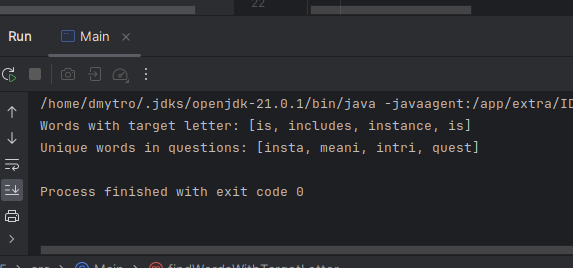
\includegraphics[scale=0.55]{1}
		\caption{Робота програми}
	\end{figure}

	\section*{Висновок}
	Під час виконання лабораторної роботи я працював з регулярними виразави. Навчився працювати з регулярними виразами.
	 
\end{normalsize}
\end{document}
